
\documentclass[10pt, conference, compsocconf,a4paper]{IEEEtran}

\usepackage[pdftex]{graphicx}

% correct bad hyphenation here
\hyphenation{op-tical net-works semi-conduc-tor}


\begin{document}
\title{Extending Mocapy++ with a mixed probability distribution\\Advanced Topics In Data Modeling}

\author{\IEEEauthorblockN{Kasper Nybo Hansen}
\IEEEauthorblockA{Dept. of Computer Science\\
University of Copenhagen\\
Copenhagen, Denmark\\
nybo@diku.dk}
}

% make the title area
\maketitle

\begin{abstract}
Mocapy++ is a C++ toolkit for learning and inference in dynamic Bayesian networks. This report describes the implementation, testing and results of extending Mocapy++ with a new node. 

The new node is a mixed node, allowing both discrete and continuous values. The continuous part of the node is a gaussian distribution. The new node is used to calculate a probabilistic model of hydrogen bonding in protein structures. The probabilistic model is learned from a provided dataset.
\end{abstract}

\begin{IEEEkeywords}
Mocapy++; DIKU; Dynamic Bayesian networks; Mixed probability distribution
\end{IEEEkeywords}


\section{Introduction} % (fold)
\label{sec:introduction}

% http://www.stat.uiowa.edu/~nshyamal/22S175/DI.pdf
% 
% http://www.tutorvista.com/math/mixed-probability-distribution
% http://www.freemathhelp.com/forum/viewtopic.php?f=12&t=34692
% 
% Good explanation
% http://www.ds.unifi.it/VL/VL_EN/dist/dist3.html

An introduction with a short discussion of the theory of inference and learning in Bayesian networks, relevant to Mocapy++.

When using the mixed node in hydrogen bondings, the following 

\subsection{Dynamic Bayesian Network} % (fold)
\label{sub:dynamic_bayesian_network}
A Bayesian network consists of a Directed Acyclic Graph where the nodes are probability distributions depended on the pare
% subsection dynamic_bayesian_network (end)


\subsection{Mixed distribution} % (fold)
\label{sub:mixed_distribution}
The mixed distribution can be divided into two parts. A discrete and continuous part. Let $X$ be a random variable that takes values in the set $S$. We then define the discrete part as the countable set $D \subseteq S$, and the continuous part as $C \subseteq S$. We define a mixed distribution as a distribution that has the following two probabilities

\begin{itemize}
  \item $0 < P(x \in D) < 1$
  \item $P(x \in C) = 0$
\end{itemize} 
% subsection mixed_distribution (end)

\subsection{Applications to Hydrogen bounding} % (fold)
\label{sub:applications_to_hydrogen_bounding}
The mixed distribution applies to hydrogen bonding in the following way. A hydrogen bound has two states:

\begin{itemize}
  \item A bond does not exist
  \item A bond exists with a energy $E$
\end{itemize}

Under the assumption that the energy of a hydrogen bonding can be modeled by a Gaussian probability distribution we can model a hydrogen bond in the following way. The discrete distribution is modeling the first boolean case, i.e. "Is the bond present or not?". If the bond is present, the Continuous part can be used to to find the energy, $E$, of the bond.

% subsection applications_to_hydrogen_bounding (end)


% section introduction (end)

\section{Implementation} % (fold)
\label{sec:implementation}
A description of the implementation of the mixed distribution in Mocapy++. 

We assume that the parent node can only take one value

A mixed node has the following parameters, CPD, mean and variance. The CPD determines the relationship between the continuous and discrete distribution. It is a table of probabilities, where.

The mean and variance is parameters used in the continuous part of the distribution, more precisely in the Gaussian distribution. 
                                                                                                                                  

When instantiating a new node, it is possible to ask the node to take on random values. Furthermore it is possible to specify the CPD, mean and variance. If nothing is specified the node is initialized with a uniformly distributed CDP, and random values for the mean and variance. 




\subsection{ESS} % (fold)
\label{sub:ess}
ESS
%subsection ess (end)

\subsection{Densities} % (fold)
\label{sub:densities}
CPD = 2*parent size, each parent can yield a value, the indicator shows if it is continuous or discrete

The sampling returns a tuple where the first value is the indicator, and the second is the energy.

% subsection densities (end)
%section implementation (end)

\section{Testing of implementation} % (fold)
\label{sec:testing_of_implementation}

A description of some simple tests that show that the implementation is correct. 

\subsection{Test of inference} % (fold)
\label{sub:test_of_inference}

% subsection test_of_inference (end)

\subsection{Test of sampling} % (fold)
\label{sub:test_of_sampling}
In this test I would like to confirm that the samples drawn from the mixed node corresponds to the nodes parameters.

In \texttt{examples/hmm\_mixed2.cpp} I have made a test of the sampling part of the mixed node. I have made the test by creating a DBN with randomly picked CPD, mean and variance. I have then sampled from this network yielding data points I can use to train a second network.

The 

In order to test the sample function, I have exported the sampled data points and made two histograms. The first histogram illustrates the discrete distribution, i.e. the contents of the CPD. This normalized histogram should resemble the randomly picked CPD.

The histogram should approximate a bell curve with mean and variance corresponding what is randomly generated. The histogram can be seen on figure \ref{fig1}. On top of the histogram, is plotted a Gaussian probability density function with the mean and variance equal to the randomly generated. As can be seen from the figure \ref{fig1} the histogram approxmiates the Gaussian well, and the conclusion must be that the samples drawn from the continuous part of the distribution is correct.

\begin{figure}
\centering
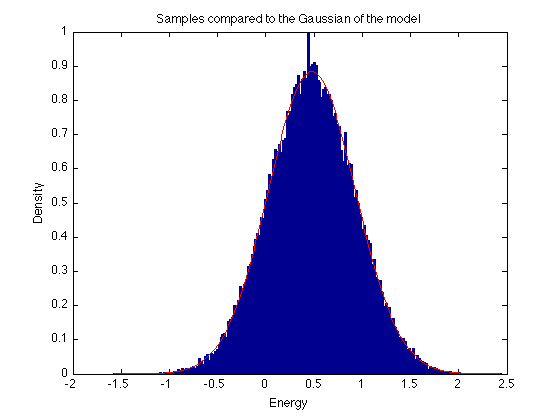
\includegraphics[width=0.5\textwidth]{figures/fig1.png}
\caption{Illustration of the samples drawn from the Gaussian part of the mixed distribution}
\label{fig1}
\end{figure}

%subsection test_of_sampling (end)

% section testing_of_implementation (end)

\section{Future work} % (fold)
\label{sec:future_work}
The present implementation does not enable the user to specify which distributions should be part of the mixed node. Future work could involve making use of the existing distributions and using them in the mixed node. This would remove the duplicate code that is present in the current prototype of the mixed node, and make the mixed node more flexible.
% section future_work (end)


\section{Results} % (fold)
\label{sec:results}

% section results (end)   



\bibliographystyle{abbrv}
\bibliography{bibliography}
\end{document}